\documentclass[a4paper, 12pt, titlepage]{article}
%=======Unpackage Things===============
\usepackage{color}
\usepackage{colortbl}
\usepackage{mathrsfs}

\usepackage{graphicx}
\usepackage{amsthm}
\usepackage{listings}
%\usepackage{fullpage}
\usepackage{epsfig}
\usepackage{amsmath}
\usepackage{latexsym}
\usepackage{amssymb}
\usepackage{amstext}
\usepackage{array}
\usepackage{titlesec}
\usepackage{float}

\titleformat{\section}
    {\normalfont\fontsize{12}{15}\bfseries}{\thesection}
    {1em}{}

%\titleformat{\subsection}
%    {\normalfont\fontsize{5}{5}\bfseries}{\thesection}
%    {1em}{}
\newcommand{\PreserveBackslash}[1]{\let\temp=\\#1\let\\=\temp}
\newcolumntype{C}[1]{>{\PreserveBackslash\centering}p{#1}}
\newcolumntype{R}[1]{>{\PreserveBackslash\raggedleft}p{#1}}
\newcolumntype{L}[1]{>{\PreserveBackslash\raggedright}p{#1}}


\begin{document}
%==title==
\title{COMP6321 Assignment 3}
\setcounter{tocdepth}{2}
\newpage
\begin{center}
    {\huge COMP6321: Assignment \#3}


    \vspace{2cm}
    Student: Qing Gu  \hspace{5cm}
    Student ID: 6935451
    \vspace{1cm}

    =================================================
\end{center}
\section{A Midterm Preparation Question}
\begin{enumerate}
    \item In this scenario, The best learning approach is instance-based learning. The training set in continuous space can be mapped to $\mathbb{R}^6$. We can observe that the training set is much larger than the queries. Thus, the time of training hypothesis would take more account. Instance-based learning methods, say KNN or decision tree, can fit in this situation very well since these algorithms take little time in training, and the number of features is not to much to make queries too slow. 
    \item I think multiple classes logistic regression is better. The features of a child can be highly related. To train the weights, we can assign each class a weight, and use $p(y=k|x)=\frac{exp(\theta_k^Tx}{\sum_{i=1}^Kexp(\theta_i^Tx)}$ as the probability function. The result is more readable than neural network.
    \item In this situation, there are large-scale binary data to classify and the training and prediction time is also important. As far as I'm concerned, Naive Bayes Classifier would be the best algorithm. First, we have binary input and binary output, it is very easy to fit in. Second, whether a person like it or not like it are mostly independent, so this will give a relatively accurate prediction.
    \item Because of the lack of training data, I would suggest SVM. SVM with feature mapping can expand the feature area which could make better prediction.
\end{enumerate}
\section{Properties of Entropy}
\begin{enumerate}
\item Evaluating Entropies

According to the given joint probability, we can come out with the following probability:
$$p\{x=1\} = \frac{1}{3}; p\{x=0\} = \frac{2}{3}$$
$$p\{y=1\} = \frac{2}{3}; p\{y=0\} = \frac{1}{3}$$
According to the entropy euqations:
$$ H[x] = \Sigma_{i=1}^np(x_i)I(x_i)=-\Sigma_{i=1}^np(x_i)\log{p(x_i)}$$
$$ H[Y|X] = \Sigma_{x\in{}X, y\in{}Y}p(x,y)\log{\frac{p(x)}{p(x,y)}}$$
$$H[Y|X]=H[X,Y]-H[X]$$
$$I[X,Y] = \Sigma_{y\in{}Y, x\in{}X}p(x,y)\log{\frac{p(x,y)}{p(x)p(y)}}$$
The following entropies and information can be calculated
\begin{itemize}
    \item $H[x] = -(\frac{1}{3}\log{\frac{1}{3}}+\frac{2}{3}\log{\frac{2}{3}})=\log{3}-\frac{2}{3}\log{2}$
    \item $H[y] = -(\frac{1}{3}\log{\frac{1}{3}}+\frac{2}{3}\log{\frac{2}{3}})=\log{3}-\frac{2}{3}\log{2}$
    \item $H[y|x] = \frac{2}{3}\log{\frac{2/3}{1/3}}+\frac{1}{3}\log{\frac{1/3}{1/3}}=\frac{2}{3}\log{2}$
    \item $H[x|y] = \frac{2}{3}\log{2}$
    \item $H[x,y] = H[y|x] + H[x] = \log{3}$
    \item $I[x,y] = H(x) - H(x|y) = \log{3} - \frac{4}{3}\log{2}$
\end{itemize}
\item Maximum Entropy Discrete Distribution

For discrete distribution, the maximum problem can be interpreted like this:
$$\max{}\Sigma{}p_i\log{1/p_i}$$
$$w.r.t~\Sigma{}p_i=1$$
Form the Lagrangian:
$$L(P, \lambda) = \Sigma{}p_i\log{1/p_i} + \lambda{\Sigma{}p_i-1}$$
Let $\frac{\delta}{\delta\lambda}L=0$ we get $\Sigma{}P_i=1$. This is the original constraint which is irrelevant with $\lambda$.

Let $\frac{\delta}{\delta{}p_j}L=0$ (Probability of an arbitrary event), we get $p_j = 2^{\lambda-1}$. Thus, entropy reaches its maximum the probability when every event is equal to a same constant. So the maximum entropy of a discrete probability is achieved for a uniform distribution.

\item Proof of T1
            \begin{figure}[H]
                \centering
                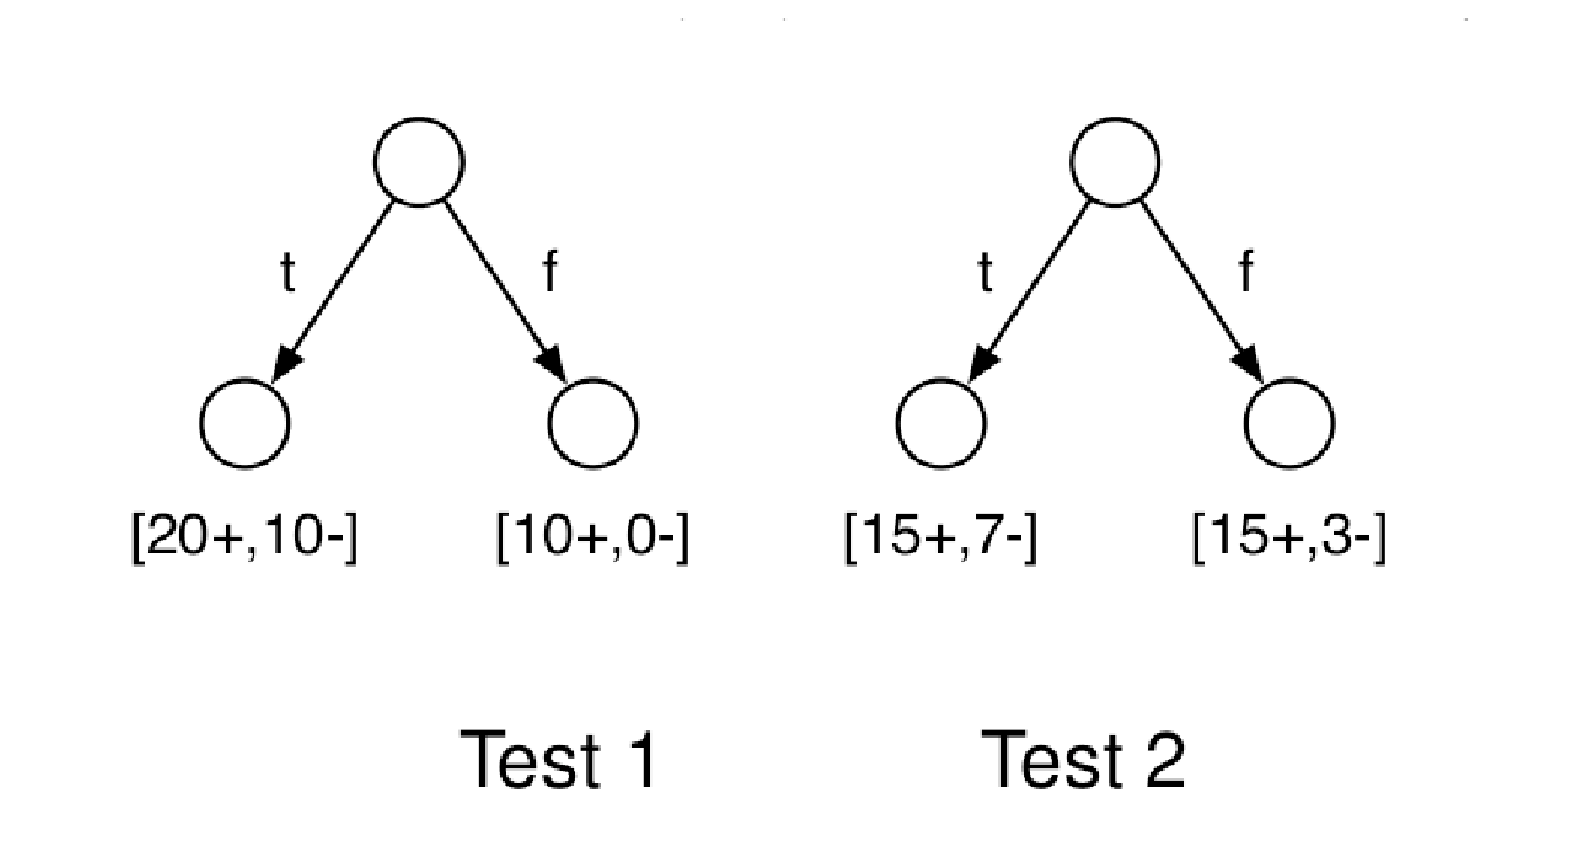
\includegraphics[width=12cm]{tests.eps}
                \caption{Tow Tests}\label{tests}
            \end{figure}

In order to prove T1 is better than T2, we have to prove that Test 1 gained more information. $IG(D|Test1)$ and $IG(D|Test2)$ are computed separately.
        $$H(D) = \frac{3}{4}\log{\frac{4}{3}}+\frac{1}{4}\log{4}=2-\frac{3}{4}\log{3}\approx0.811~bits$$
\begin{itemize}
        \item Information Gain of Test 1
            $$H(D|Test1) = \frac{3}{4}(\frac{1}{3}\log{3} + \frac{2}{3}\log{\frac{3}{2}})+\frac{1}{4}\times0 \approx 0.689~bits$$
            $$IG(D,Test1) = H(D) - H(D|Test1) \approx 0.123$$
        \item Information Gain of Test 2
            $$H(D|Test2) = \frac{22}{40}(\frac{15}{22}\log{\frac{22}{15}} + \frac{7}{22}\log{\frac{22}{7}}) + \frac{18}{40}(\frac{15}{18}\log{\frac{18}{15}} + \frac{3}{18}\log{\frac{18}{3}})\approx 0.789~bits$$
            $$IG(D,Test2) = H(D) - H(D|Test1) \approx 0.022$$
\end{itemize}
Obviously, the information gain of test 1 is higher than test 2, thus, we can come up with the conclusion that test 1 is better than test 2.
\end{enumerate}

\section{Kernels}
\begin{enumerate}
    \item $K(x,z) = aK_1(x,z) + bK_2(X,z)~ a,b>0$

        Using Merceris Theorem:

        Since $K_1$, $K_2$ are kernels, $K_{1ij} = K_{1ji}$, $K_{2ij} = K_{2ji}$. Both kernel matrices are positive semidefinite.
        $$K_{ij} = aK_{1ij} + bK_{2ij} = aK_{1ji} + bK_{2ji} = K_{ji}$$ It's symmetric.
        $$xKx^T = x(aK_1+bK_2)x^T=xaK_1x^T + xbK_2x^T$$
        Since $a,b>0$, K is positive semidefinite.
        Thus, this function is a kernel.
        
    \item $K(x,z) = aK_1(x,z) - bK_2(X,z)~ a,b>0$

        Using Merceris Theorem:

        Since $K_1$, $K_2$ are kernels, $K_{1ij} = K_{1ji}$, $K_{2ij} = K_{2ji}$. Both kernel matrices are positive semidefinite.
        $$K_{ij} = aK_{1ij} - bK_{2ij} = aK_{1ji} - bK_{2ji} = K_{ji}$$ It's symmetric.
        $$xKx^T = x(aK_1-bK_2)x^T=xaK_1x^T - xbK_2x^T$$
        Though $a,b>0$, the relationship of $xaK_1x^T$ and $xbK_2x^T$ can not be determined. $K$ is not a positive semidefinite matrix. Thus, this function is not a kernel.

    \item $K(X,Z) = K_1(X,Z)K_2(X,Z)$

        Let $K_1(X,Z) = \phi_1(X)\phi_1(Z)$ and $K_2(X,Z) = \phi_2(X)\phi_2(Z)$.
        Assume that $\phi_1(X): \mathbb{R}^n\rightarrow \mathbb{R}^a$ and $\phi_2(X): \mathbb{R}^n\rightarrow \mathbb{R}^b$.
        Then, use the definition of kernel:
        $$K(X,Z)=(\phi_1(X)^T\cdot\phi_1(Z))(\phi_2(X)^T\cdot\phi_2(Z))$$
        $$=\sum_{i=1}^a\phi_1(X)_i\phi_1(Z)_i\times\sum_{j=1}^b\phi_2(X)_j\phi_2(Z)_j$$
        $$=\sum_{i,j=1}^{a,b}(\phi_1(X)_i\phi_2(X)_j)(\phi_1(Z)_i\phi_2(Z)_j)$$
        Since $\phi_1(X)$ and $\phi_2(X)$ are given function, let $\phi=\{\phi_1(X)_i, \phi_2(X)_j\}^{i<a,j<b}$ for $K$. Thus, K is a kernel.

    \item $K(X,Z) = f(X)f(Z)$

        Using the definition of kernel function.
        $$K(X,Z) = \phi(X)\phi(Z)$$
        Then we let $\phi_1(X): \mathbb{R}^n\rightarrow \mathbb{R}$, then $\phi(X)^T=\phi(X)$.
        
        The original formula can also be written in the form of a kernel. Thus, it is a kernel.

\end{enumerate}

\section{Nearest Neighbors vs. Decision Trees}
In general, the decision boundary of 1-NN is a set of edges on a Voronoi Graph, they are vertical to the line that links two data points. And the boundary generated by decision tree, is some vertical horizontal lines in the 2D space if all of the tests are tests either on $x$ or $y$. But they can also coincide under some circumstance. 

Consider the situation in fig\ref{db}. This is a decision generated by Voronoi Graph, which indicate the decision boundary of 1-NN. 
            \begin{figure}[H]
                \centering
                \includegraphics[width=9cm]{db.eps}
                \caption{Average Training and Test Error}\label{db}
            \end{figure}
If we perform Decision Tree on this data set, the decision boundary would be as same as the 1-NN.

\section{Implementation}
In the implementation part, I performed KNN algorithm on the Wisconsin data set with 2 fold cross-validation. The metric I use is the square of Euclidean distance. Fig\ref{err} shows how the error fluctuate with K. Where K is from 1 to 35.
            \begin{figure}[H]
                \centering
                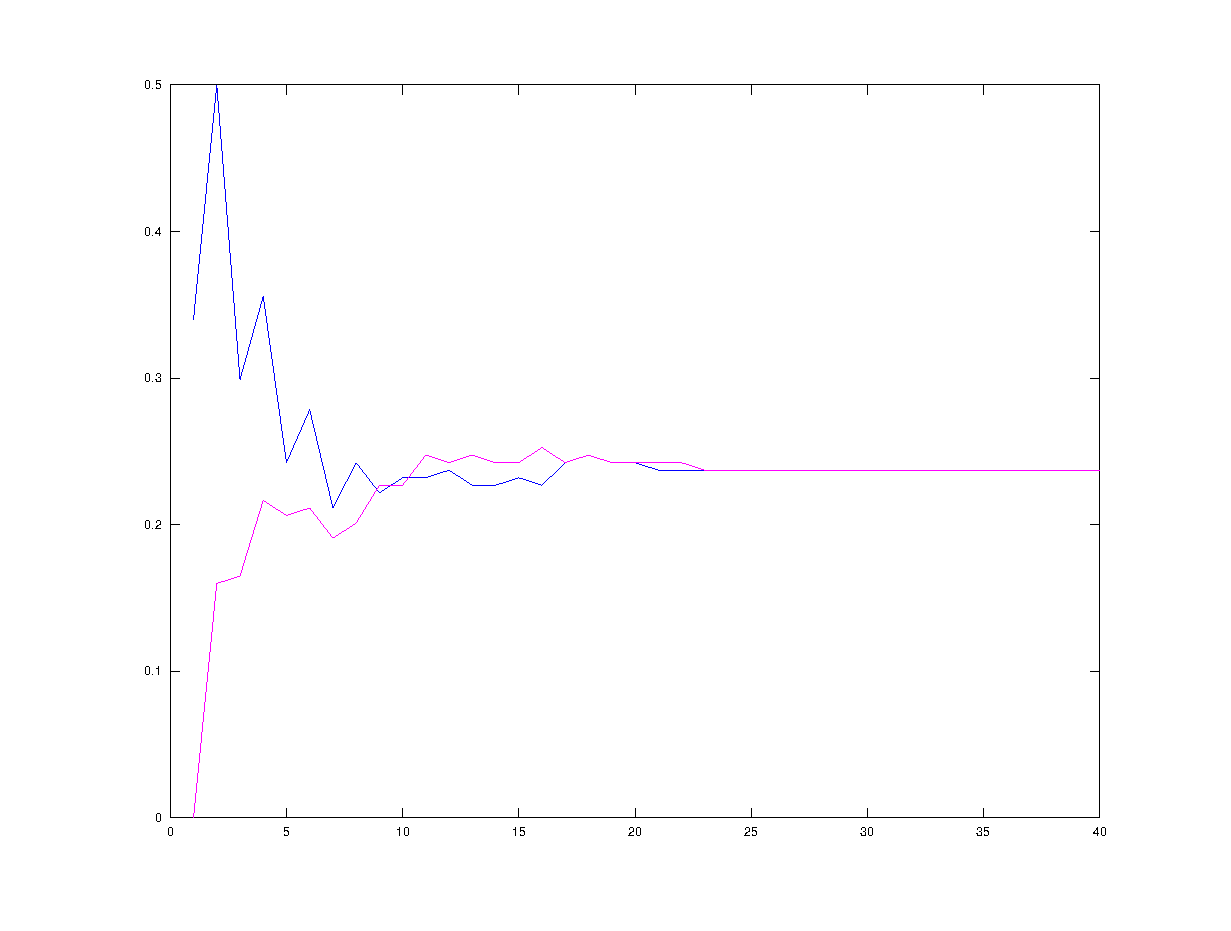
\includegraphics[width=12cm]{Q5.eps}
                \caption{Average Training and Test Error}\label{err}
            \end{figure}
In the picture, the red line denotes the average training error, and the blue line denotes the average test error.







\end{document}
